\newproblem{15E. Triangles}
\begin{prob}
	\begin{center}
		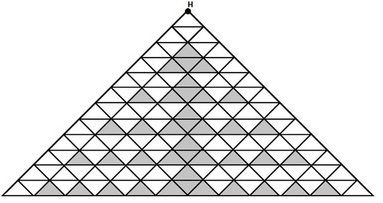
\includegraphics{15E.png}
	\end{center}
	\par
	求从$H$出发再回到$H$的路径数,满
	足不自交,且形成的封闭区域不含阴影三角形。
\end{prob}

\begin{sol}
	显然一条满足要求的路径必然是左边走
	一圈,回到最靠上阴影三角
	形的上定点,然后再在右边走一圈。
	仔细观察可以发现很多递归子问题,
	一个是往中间走然后出来,一个是往下走然后
	回去。设前者为$f[i]$,后者是$g[i]$,不难发现递推式:
	\par
	$f[1]=1$;$f[i]=2f[i-1]+3$;
	\par
	$g[n/2]=2$;$g[i]=2+2f[i]+f[i] \cdot g[i+1]$;
	\par
	答案就是$2(g[1]^2+1)$。
\end{sol}
